\documentclass[letterpaper]{article}

\usepackage{natbib,alifeconf}  %% The order is important
\usepackage{url,hyperref,cleveref}
\usepackage{booktabs}

% *****************
%  Requirements:
% *****************
%
% - All pages sized consistently at 8.5 x 11 inches (US letter size).
% - PDF length <= 8 pages for full papers, <=2 pages for extended
%    abstracts (not including citations).
% - Abstract length <= 250 words.
% - No visible crop marks.
% - Images at no greater than 300 dpi, scaled at 100%.
% - Embedded open type fonts only.
% - All layers flattened.
% - No attachments.
% - All desired links active in the files.

% Note that the PDF file must not exceed 5 MB if it is to be indexed
% by Google Scholar. Additional information about Google Scholar
% can be found here:
% http://www.google.com/intl/en/scholar/inclusion.html.


% If your system does not generate letter format documents by default,
% you can use the following workflow:
% latex example
% bibtex example
% latex example ; latex example
% dvips -o example.ps -t letterSize example.dvi
% ps2pdf example.ps example.pdf


% For pdflatex users:
% The alifeconf style file loads the "graphicx" package, and
% this may lead some users of pdflatex to experience problems.
% These can be fixed by editing the alifeconf.sty file to specify:
% \usepackage[pdftex]{graphicx}
%   instead of
% \usepackage{graphicx}.
% The PDF output generated by pdflatex should match the required
% specifications and obviously the dvips and ps2pdf steps become
% unnecessary.


% Note:  Some laser printers have a serious problem printing TeX
% output. The use of ps type I fonts should avoid this problem.


\title{\vspace{-1.5cm}Spatial sensitivity of the evolutionary swarm chemistry model}

% Each submission will undergo a double-blind review process. To this end, submissions should NOT contain any element that could reveal the identity of the authors (author names, affiliations, funding details and acknowledgments), and should use the third person to refer to previous work by the authors.
\author{
    Juste Raimbault$^{1}$\\
    \mbox{}\\
    $^1$LaSTIG, Univ Gustave Eiffel, IGN-ENSG\\
%    $^2$Second Institution Name, Second Institution Country
    juste.raimbault@ign.fr
} % email of corresponding author

% For several authors from the same institution use the same number to
% refer to one address.
%
% If the names do not fit well on one line use
%         Author 1, Author 2 ... \\ {\Large\bf Author n} ...\\ ...
%
% If the title and author information do not fit in the area
% allocated, place \setlength\titlebox{<new height>} after the
% \documentclass line where <new height> is 2.25in



% TODO camera ready
% X labels fig
% X ticks axis fig
% X stat test averages? TODO redo with better experiment
% X swarm size: 200 if better pse results: OK
% X evol swarm chem: more explicit in title abstract and intro
% X objective is not to get insight into real-world evolution (request by rev 3 to develop this) -> clarify


\begin{document}

\maketitle

% Abstract length should not exceed 250 words
\begin{abstract}
    Artificial life simulation models are most of the time spatially explicit, yet there are not much dedicated studies of how spatial structure and spatial initial conditions influence model outcomes. We propose in this contribution to study the role of spatial structure in the classical model of swarm chemistry. We couple the evolutionary swarm chemistry model with spatial structure generators, and quantify the impact of space on diversity outcomes by using a diversity search algorithm. We find a significant influence of the type of spatial structure on model outcomes.
\end{abstract}

% kws: Spatial sensitivity analysis ;Spatial context; Swarm chemistry; Diversity search
% topics: Bio-inspired, cognitive and evolutionary robotics, swarms ; Others [pas artifical chem: OoL]

\section{Introduction}

The role of spatial structure and dynamics in evolution has been highlighted \citep{lion2008self}, but remains an auxiliary focus in the literature as most models do not consider space or in very simplified settings. An evolutionary niche is not principally defined by its spatial extent, but indeed corresponds to some geographical territories, and it has furthermore been shown that spatial effects may favour niche construction \citep{silver2006spatial}. From the viewpoint of \cite{holland2012signals}'s theory for complex adaptive systems, boundaries are at the core of the niche concept and thus the spatial structure of complex systems defines their dynamics. Also, biogeography optimisation algorithms have a good performance precisely because evolution is embedded in space \citep{simon2008biogeography}. Therefore, a better understanding of the role of space is an important theoretical component for the discipline of Artificial Life.

Regarding Artificial Societies, and more particularly socio-spatial simulation models, a recent stream of work investigated this aspect. \cite{raimbault2019space} showed that spatial initial conditions could have as much impact on model outcomes than the parameters of the model itself. \cite{raimbault2023spatial} detailed how diverse spatial configuration generators can be coupled with simulation models to quantify such effects. The term of Spatial Sensitivity Analysis was coined in that context, and a specific \texttt{scala} library was developed to implement these methods \citep{raimbault2020scala}. A question remaining open is to what extent such effects are specific to social systems, or do they hold in other disciplines. Furthermore in terms of broader methodological aspects, sensitivity analysis of ALife models is not widely applied despite a few examples such as \citep{alden2014easing}.

This contribution reports on preliminary results aimed at investigating the spatial sensitivity in ALife simulation models. More particularly, we focus on an iconic model of ALife which is the Swarm Chemistry model \citep{sayama2009swarm}. It is a well studied model of self-organisation, and it was shown by \citep{sayama2018seeking} that introducing evolutionary dynamics between particles could generate swarm patterns in an open-ended way. While \citep{sayama2018seeking} uses space to introduce evolutionary pressure through perturbations and shows that evolution outcomes are strongly influenced by the magnitude of the perturbation, it remains a simple splitting of the world in half. We couple the evolutionary version of the model with more elaborate spatial structure generators for the spatial distribution of competition rules, and investigate the role of the spatial structure on diversity outcomes.

\section{Methods}

We use the evolutionary version of Swarm Chemistry described by \citep{sayama2018seeking}. The base of the model are particles which self-organise based on local interaction rules (on speed and rotation e.g.) ruled by particle-level parameters. Some mutation in parameter values and transmission between particles at collision allows some evolutionary dynamics to be introduced. As no global fitness landscape rules this evolution, different rules can be used for this ``selection'' step at transmission: faster particle transmits its genome, slower transmits, the majority within a local neighbourhood is taken, etc. These rules can be changed in space and time to foster evolutionary dynamics as shown by \citep{sayama2018seeking}.

We introduce a spatial context in which swarm dynamics and evolution will take place. Given a grid decomposition of the two dimensional space (in practice with a lower resolution than coordinates), each cell of the grid will contain the transmission rule for collisions occurring in this cell. We consider the rules ``Faster'', ``Slower'', ``Behind'', ``Majority'' and ``Majority Relative'' only (see \citep{sayama2018seeking} for details), and organise the spatial distribution of rules with some structure. We use the following spatial contexts: (i) a totally random attribution of cell rule, to act as a null model (``random''); (ii) a uniform rule chosen randomly among all rules - which should also be a null model in some sense (``uniform''); (iii) four rectangular quadrants, with the space being split at a random x coordinate and at a random y coordinate, and with a uniform random rule within each quadrant - this configuration corresponds to neighbour regions with different evolution dynamics and exchanging particles, in a similar way to biogeography algorithms (``split''); (iv) a more realistic hierarchical organisation, inspired by the spatial organisation of systems of cities \citep{batty2008size}: a certain number of ``urban centres'' ($C=10$ in practice) with a scaling law distribution of sizes (Zipf's law, with a scaling exponent $\alpha_C = 1$ \citep{pumain2006evolutionary}) are randomly distributed in space, an exponential kernel with a radius proportional to the size is applied for each centre (monocentric cities \citep{lemoy2020evidence}), the distribution is rescaled as a probability distribution, a threshold ($\theta_C = 0.5$ in practice) is applied to discriminate between inside and outside of centres, and finally a randomly chosen rule is applied inside and an other random rule outside (``zipf''). Although inspired by urban science and patterns in social systems, we believe this last generator could also capture existing natural structures with similar hierarchical distributions, and have some genericity since hierarchy is recurrent in natural and social complex systems \citep{pumain2006hierarchy}.

We focus on the diversity of particles as an outcome of coupling the spatial generators with swarm dynamics, as it is a key aspect for evolution and open-ended systems. We consider average and standard deviation of three particle parameters, namely $c_1, c_2, c_3$ which capture the main essence of each particle behaviour. This gives a 6-dimensional output, for which we seek to maximise diversity using the Pattern Search Exploration algorithm developed by \citep{cherel2015beyond}.

Swarm parameters are fixed at their default values used in \citep{sayama2018seeking}, except for swarm size taken smaller for performance reasons ($N=200$), and final time $t_f = 10000$. The swarm is initialised with 20 random individuals and 180 inactive particles. The free parameters for the diversity search algorithm, run for 2100 generations, are the seed of the random number generator, and the type of spatial generator used among the four described above.
%After 1000 generations less patterns are discovered and the algorithm is stopped.
% %except for mutation at normal time which was increased to 0.5 -> TODO future work: influence of other parameters

\section{Results}

We use the implementation of spatial structure generators provided by \citep{raimbault2020scala}. For an easier integration with this scala library, the Swarm Chemistry model was reimplemented in scala, based on the open source Java code provided by \citep{sayama2018seeking}. Our implementation is embedded into the OpenMOLE software for exploration and validation of simulation models \citep{reuillon2013openmole}, which includes the PSE diversity search algorithm. Source code and results are available on an open git repository at \url{https://github.com/JusteRaimbault/SwarmChemistrySpatialSensitivity}.


\begin{figure}
    \centering
    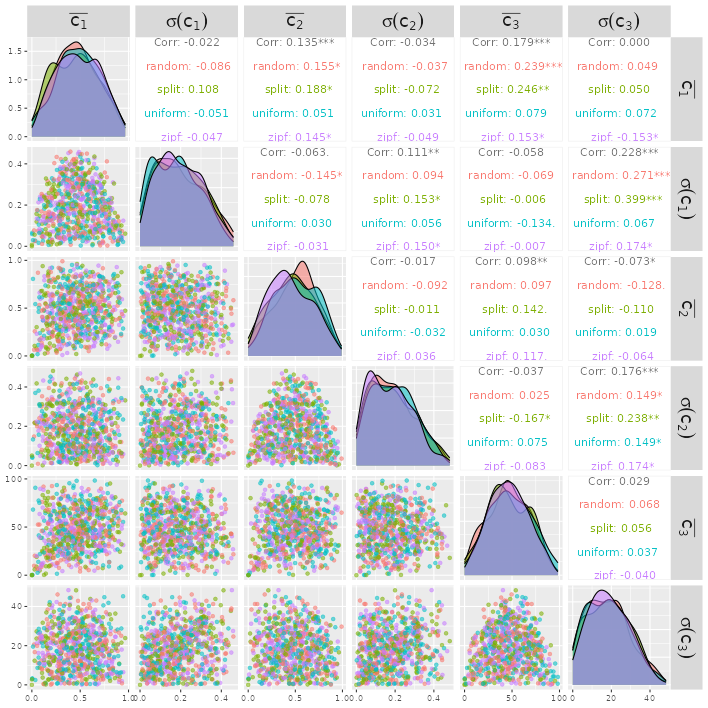
\includegraphics[width=\linewidth]{figures/pse-scatterplot_colorGenerator.png}
    \caption{Scatterplot of PSE objectives, with points coloured by type of generator. Running t-tests between group averages for each indicator yields p-values smaller than 0.1 for $\sigma(c_1)$ (between uniform and zipf) and for $\bar{c_2}$ (zipf-random, zipf-uniform, uniform-split).}
    \label{fig:pse}
\end{figure}
% TODO more stat tests differences: manova

% TODO other experiment: param values where effect of space is stronger?

We show in Fig.~\ref{fig:pse} scatterplots of the final point cloud obtained with the PSE algorithm. The overall shape of each plot is not trivial, with reduced standard deviations for averages values of averages for each parameters. Correlation patterns are also diverse. When comparing across generators (point colour), statistical distribution are significantly changing for some dimensions, for example $\sigma(c_1)$ (which shows a unique bimodal distribution for zipf only) and $\bar{c_2}$, what is confirmed by t-test values (see legend of Fig.~\ref{fig:pse}). When looking at the stronger and most significant correlations, between $\bar{c_1}$ and $\bar{c_3}$, only uniform space is not significant and close to zero, while other are high.
%We also compare hypervolumes
%Simple linear models to link the type of generator with outputs
Altogether, these results confirm a significant effect of the spatial context on evolution outcomes in this model.

% distrib
%  random   split uniform    zipf 
%    134     120     122     118 

% hypervolumes


\section{Discussion}

% more realistic generators / in link with chem? cf cities - application to ecology
% heterogenous mutation rates? - observe migration of particles? - biogrography in practice?

We show the important influence of space in a typical Artificial Life model with these preliminary results. Note that this work was not aimed at informing real-world evolutionary processes, but rather to open a methodological research direction on spatial sensitivity analysis of ALife models. Future work will have to focus on better understanding how qualitatively each structure influences evolution, and trying to observe recurrent evolutionary patterns such as potentially the emergence of a particle biogeography. Other types and more realistic generators for this particular system, but also the application to other disciplines such as ecology and possibly more realistic evolutionary processes, are also important future research directions.

\footnotesize
\bibliographystyle{apalike}
\bibliography{biblio.bib} % replace by the name of your .bib file



\end{document}



\begin{figure}
    \centering
    \includegraphics[width=2.1in,angle=-90]{}
    \caption{}
    \label{fig1}
\end{figure}




\begin{table}[ht]
    \centering
    \begin{tabular}{cccc}
        \toprule
        Name & Result & Bonus $b_i$ & Difficulty\\
        \midrule
        Echo & I/O   & 1 & --\\
        Not  & $\neg A$ & 2 & 1 \\
        Nand & $\neg(A\wedge B)$ & 2 & 1 \\
        Not Or & $\neg A \vee B$ & 3 & 2 \\
        And  &  $ A \wedge B $   & 3 & 2 \\
        Or   &  $ A \vee B $     & 4 & 3 \\
        And Not & $A\wedge\neg B$& 4 & 3 \\
        Nor  & $\neg(A\vee B)$   & 5 & 4 \\
        Xor  & $ A\ {\rm xor}\ B$ &   6 & 4 \\
        Equals &$\neg(A\ {\rm xor}\ B)$&6& 4 \\
        \bottomrule
    \end{tabular}
    \caption{
        Logical calculations on random inputs $A$ and $B$ rewarded,
        bonuses, and difficulty (in minimum number of {\tt nand} instructions
        required). Bonuses $b_i$ increase the speed of a CPU by a factor
        $\nu_i=1+2^{b_i-3}$.
    }
\end{table}
